\chapter{Business Process Modeling}

\textbf{Business process management} is the systematic method of examining an organization's existing business processes and implementing improvements to make its workflow more effective and efficient (IBM made a fortune with business process management). A \textbf{business process} is a set of business activities that represent the required steps to achieve a business objective. A \textbf{business process model} (Figure \ref{fig:business-model-example}) consists of a set of activity models and execution constraints among them. A \textbf{business process instance} represents a concrete case in the operational business of a company, consisting of activity instances.

\begin{figure} [H]
    \centering
    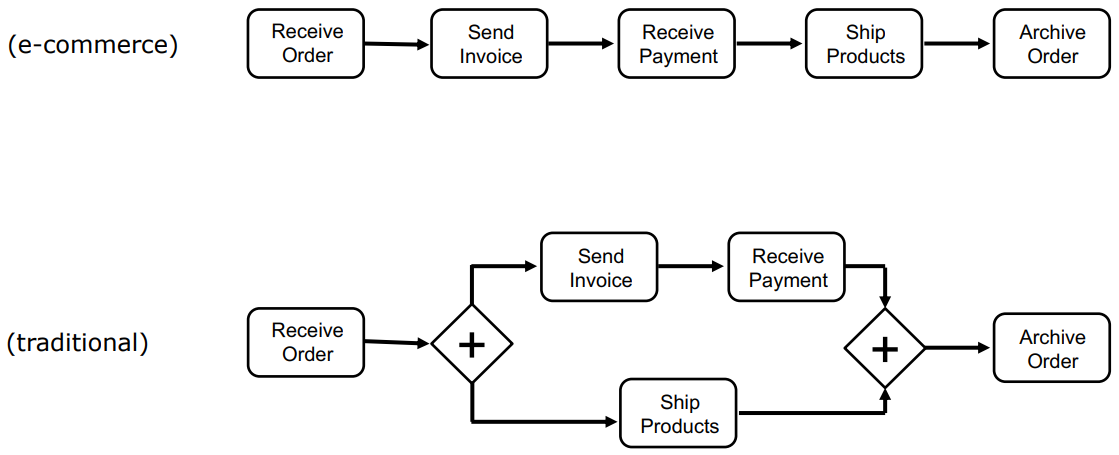
\includegraphics[width=1\textwidth]{images/BusinessProcessModeling/business-model-example.PNG}
    \caption{Example of a business process model}
    \label{fig:business-model-example}
\end{figure} 

\section{BPMN}

\textbf{Business Process Model and Notation} (BPMN) is the graphical notation for business process modeling, as shown in Figure \ref{fig:BPMN}.

\begin{figure} [H]
    \centering
    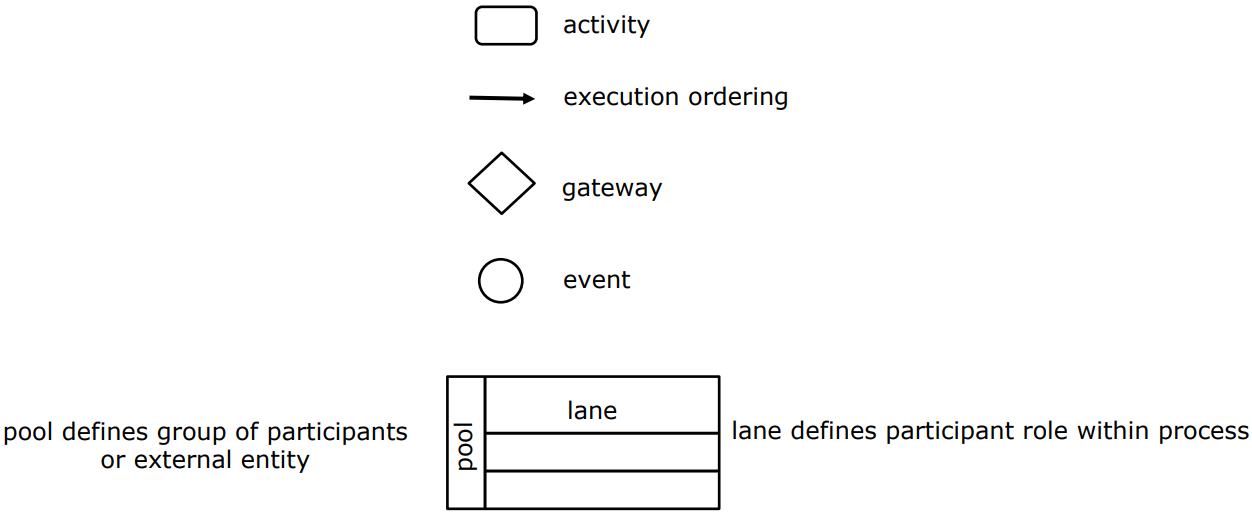
\includegraphics[width=1\textwidth]{images/BusinessProcessModeling/BPMN.PNG}
    \caption{Graphical notation for business process modeling}
    \label{fig:BPMN}
\end{figure} 

\noindent An example of a complete BPMN is shown in Figure \ref{fig:BPMN-ship}. This example demonstrates how \textbf{parallel gateway}, \textbf{exclusive gateway}, and \textbf{inclusive gateway} work.

\begin{figure} [H]
    \centering
    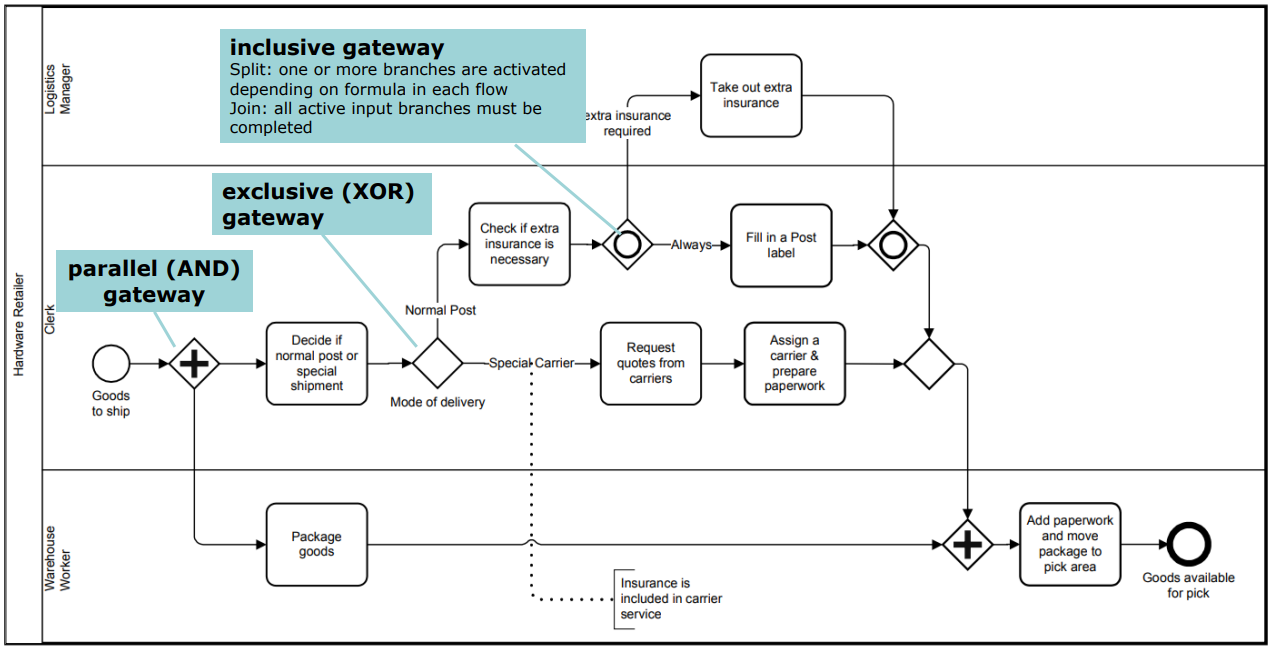
\includegraphics[width=1\textwidth]{images/BusinessProcessModeling/BPMN-ship.PNG}
    \caption{Shipment process of hardware retailer example}
    \label{fig:BPMN-ship}
\end{figure} 

\noindent Another example is shown in Figure \ref{fig:BPMN-pizza}, where we can see how multiple processes can interact with each other using \textbf{message flow}. As we can see, there is a main process and a secondary one. When a \textbf{terminate event} is reached, all activities in the process immediately end. In the main process, we also see a \textbf{timer event} and an \textbf{event-based gateway}.

The last example in Figure \ref{fig:BPMN-order} shows the \textbf{sub-process} notation and the \textbf{attached event} notation (both error $\rightarrow$ interrupting and escalation $\rightarrow$ non-interrupting).

\begin{figure} [H]
    \centering
    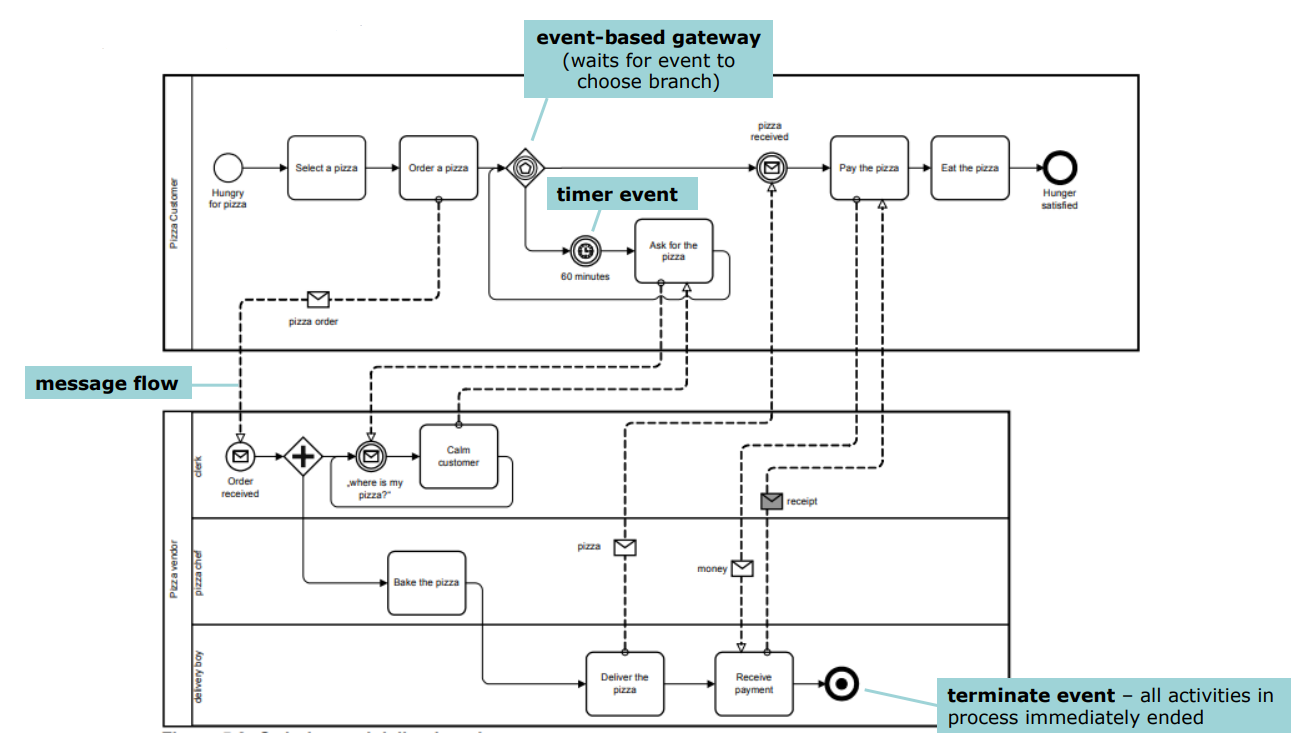
\includegraphics[width=1\textwidth]{images/BusinessProcessModeling/BPMN-pizza.PNG}
    \caption{B2B (pizza) collaboration example}
    \label{fig:BPMN-pizza}
\end{figure} 

\begin{figure} [H]
    \centering
    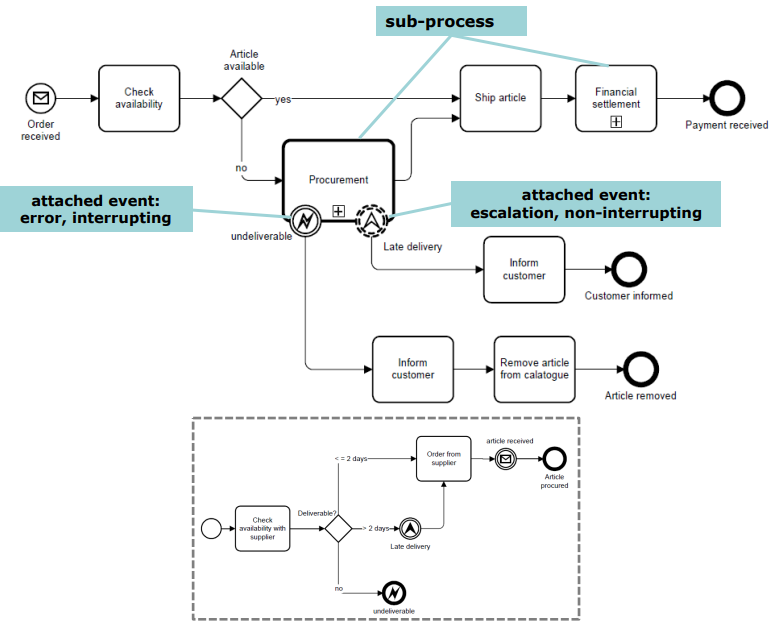
\includegraphics[width=1\textwidth]{images/BusinessProcessModeling/BPMN-order.png}
    \caption{Order fulfillment and procurement example}
    \label{fig:BPMN-order}
\end{figure} 

\noindent The ability to \textbf{prove properties of business process models is crucial} in business process management.

\section{Workflow Nets}

Workflow nets are an extension of \textbf{Petri nets}, and they are one of the best-known techniques for specifying business processes in a formal and abstract way. The graphical representation of Petri nets \textit{eases communication} between different stakeholders. \textbf{Process properties can be formally analyzed}, with the support of various tools that are available.

Figure \ref{fig:petri-nets-example} shows how Petri nets ease the reading of a business process model, translating the example shown in Figure \ref{fig:business-model-example}.

\begin{figure} [H]
    \centering
    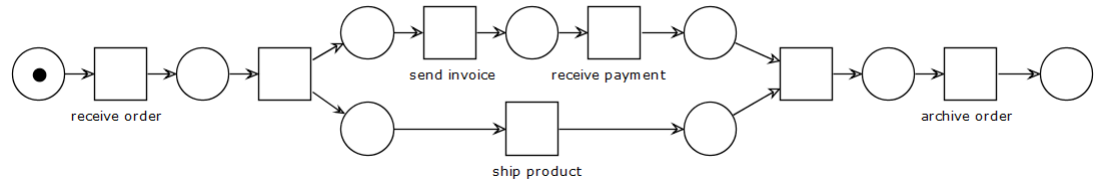
\includegraphics[width=1\textwidth]{images/BusinessProcessModeling/petri-nets-example.PNG}
    \caption{Petri net of the previous BPM example (Figure \ref{fig:business-model-example})}
    \label{fig:petri-nets-example}
\end{figure} 

Petri nets consist of \textbf{transitions} (squares), \textbf{places} (circles), and direct \textbf{arcs} connecting places and transitions. Transitions model activities, and places and arcs model execution constraints. System dynamics are represented by \textbf{tokens}, whose distribution over the places determines the state of the modeled system. A transition \textit{can fire} if there is a token in each of its input places, as shown in Figure \ref{fig:petri-nets-input}.

\begin{figure} [H]
    \centering
    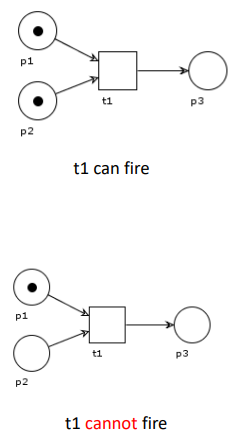
\includegraphics[width=0.3\textwidth]{images/BusinessProcessModeling/petri-nets-input.PNG}
    \caption{Petri nets input rule}
    \label{fig:petri-nets-input}
\end{figure} 

If a transition \textit{fires}, one token is removed from each input place and one token is added to each output place, as shown in Figure \ref{fig:petri-nets-output}.

\begin{figure} [H]
    \centering
    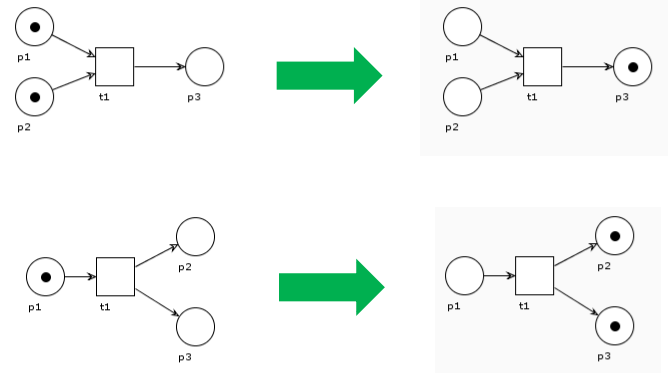
\includegraphics[width=0.8\textwidth]{images/BusinessProcessModeling/petri-nets-output.PNG}
    \caption{Petri nets output rule}
    \label{fig:petri-nets-output}
\end{figure} 

The concept of \textbf{workflow nets} enhances Petri nets with notations that simplify the representation of business processes. Like Petri nets, workflow nets focus on the control flow behavior of a process: \textbf{transitions} represent activities, \textbf{places} represent conditions, and \textbf{tokens} represent process instances. Figure \ref{fig:composition-patterns} shows some composition patterns that can be used with Petri nets.

\noindent \textit{A Petri net is a \textbf{workflow net} if and only if}:
\begin{enumerate}
    \item There is a unique source place with no incoming edge.
    \item There is a unique sink place with no outgoing edge.
    \item All places and transitions are located on some path from the initial place to the final place.
\end{enumerate}

\noindent \textit{A workflow net is \textbf{sound} if and only if}:
\begin{enumerate}
    \item Every net execution starting from the initial state (one token in the \textbf{source place}, no tokens elsewhere) eventually leads to the final state (one token in the \textbf{sink place}, no tokens elsewhere).
    \item Every transition occurs in at least one net execution.
\end{enumerate}

Notice that workflow nets abstract from data, meaning that data-dependent choices are modeled as ``blind'' choices. As a consequence, the analysis may consider “more branches than needed.” This means that a \textit{not sound workflow net} \textbf{must be interpreted only as a “warning”} of possible problems that may arise at runtime (e.g., the analysis of a branch that will never be executed may determine that the net is not sound, even if the application will never execute such a branch). \newline \noindent Conversely, the analysis of an iteration may fail to determine that the application will never terminate: a \textit{sound workflow net} \textbf{cannot be interpreted as a guarantee} that the application will always terminate its execution.

\begin{figure} [H]
    \centering
    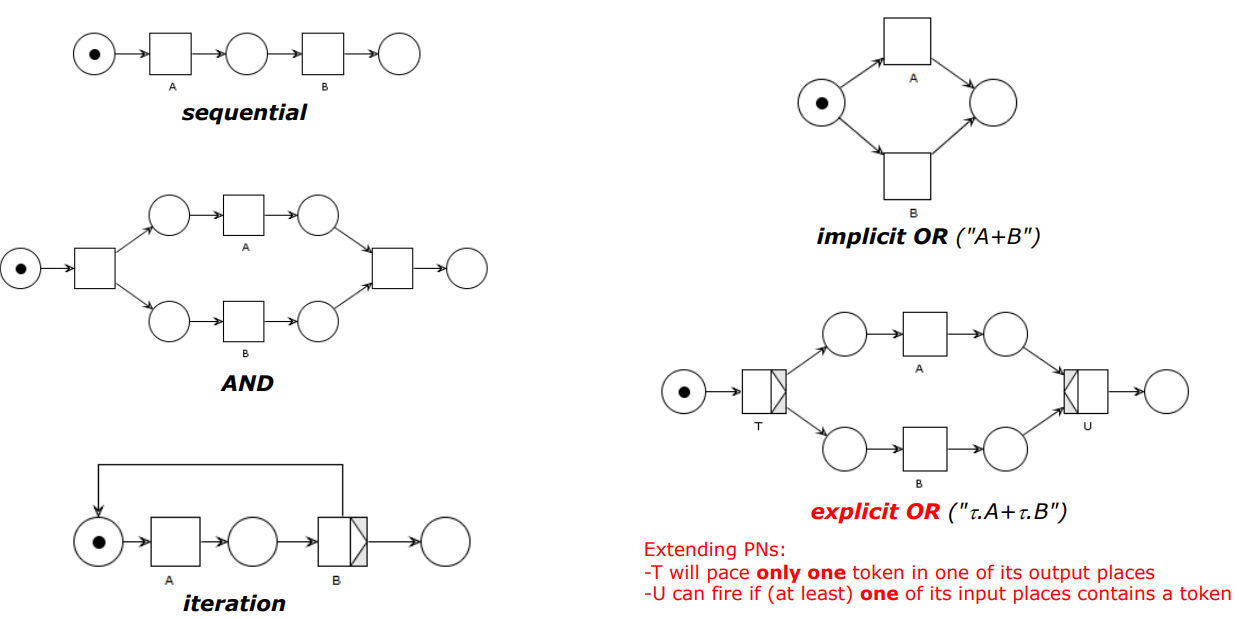
\includegraphics[width=0.97\textwidth]{images/BusinessProcessModeling/composition-patterns.PNG}
    \caption{Petri nets composition patterns}
    \label{fig:composition-patterns}
\end{figure} 

\noindent How can we formally (and automatically) establish whether a net is sound? We first need to define a couple of properties:
\begin{itemize}
    \item A Petri net ($PN$, $M$) is \textbf{\textit{live}} if and only if for every reachable state $M'$ and every transition $t$, there is a state $M''$ reachable from $M'$ where $t$ is enabled.
    \begin{figure} [H]
    \centering
    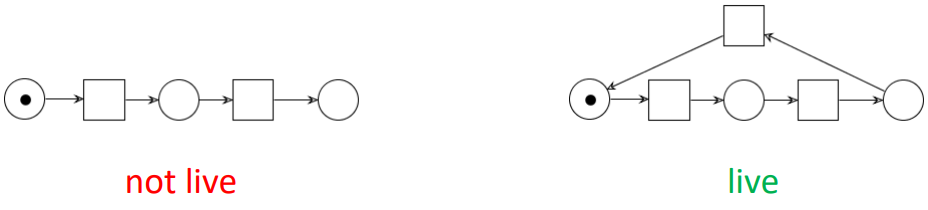
\includegraphics[width=0.69\textwidth]{images/BusinessProcessModeling/live.PNG}
    \end{figure} 
    \item A Petri net ($PN$, $M$) is \textbf{\textit{bounded}} if and only if for every place $p$ there is an $n \in \mathbb{N}$ such that for each reachable state $M'$, the number of tokens in $p$ in $M'$ is less than $n$.
    \begin{figure} [H]
    \centering
    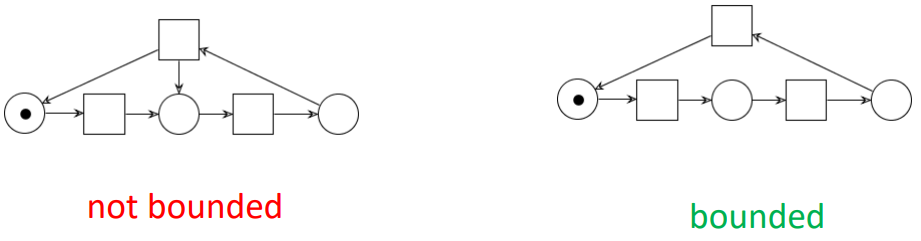
\includegraphics[width=0.69\textwidth]{images/BusinessProcessModeling/bounded.PNG}
    \end{figure} 
\end{itemize}

\noindent \textbf{Theorem}: A workflow net $N$ is sound if and only if ($\check{N}$, $\{i\}$) is live and bounded, where $\check{N}$ is $N$ extended with a transition from the sink place $o$ to the source place $i$
